\chapter{Variational quantum eigensolver}\label{ch:vqe}
At first glance, the term variational quantum eigensolver may seem complicated and it does not say anything to people outside of quantum computing. Thus, the objective of this chapter is to provide a clear explanation of the variational quantum eigensolver and clarify why it is termed as it is. For the rest of this thesis, we will use the abbreviation VQE.

The VQE is a hybrid algorithm that attempts to find eigenvalues of Hamiltonian. The term ''hybrid'' refers to a scenario where part of the algorithm runs on a quantum computer and part of the algorithm runs on a classical computer.

\begin{figure}[H]
    \centering
    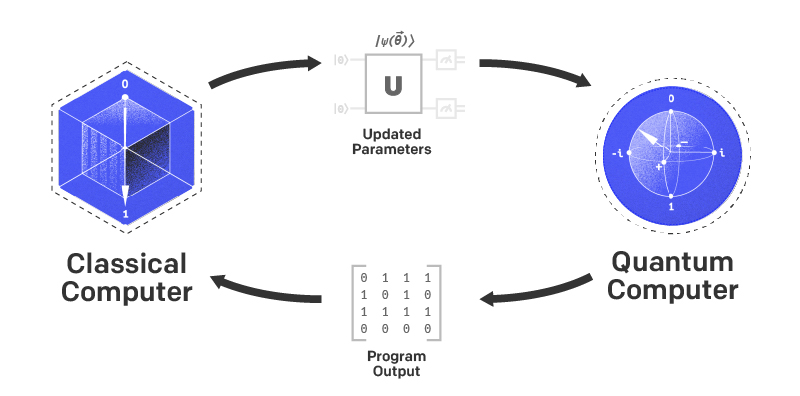
\includegraphics[width=\textwidth]{vqe.jpeg}
    \caption{Hybrid algorithm that runs on both quantum and classical computers~\cite{hybrid_alg}}
\end{figure}

Apart from VQE, there are other algorithms that can solve from eigenvalues. One of them is the quantum phase estimation algorithm (QPE). QPE is purely a quantum algorithm that imposes significant requirements on quantum hardware and that will be not possible in the near future. This problem led to the introduction of VQE. VQE tries to reduce the demands on resources, by shifting part of the work to standard computers.~\cite{fedorov2021vqe}

In this thesis, we deal with finding the ground state energy of a molecule. Arguably, this is the most prominent use case, but this is not the one and only application of VQE. It can be used for any problem that can be mapped to Hamiltonian expression. For instance, in the area of finance, it can be a portfolio optimization problem.

\section{Variational principle}
In quantum mechanics, there is a famous Schrödinger equation ($\hat{H} \Psi = E \Psi$)\ques{is it necessary to explain what the individual terms are?}, which is a partial differential equation that describes how the quantum state of a physical system behaves. Solving this equation analytically \todo{maybe explain what does analytically mean?} is really hard, in most cases, we must resort to computers to determine the solutions. This imposes very high time and memory requirements on computers, therefore we rely on the variational method which gives us an approximation of the ground state energy of a quantum system and enables us to solve the problem much more efficiently.~\cite{Thijssen_2007}

From the computer science standpoint, it is enough to know that it is an approximation method to find the ground state energy of a quantum system.

\section{Eigensolver}
As we indicated above, this algorithm solves for eigenvalues of a given Hamiltonian. Specifically, we are interested in the lowest eigenvalue because that eigenvalue corresponds to the ground state energy. 

Let $\hat{H}$ be our Hamiltonian, $\Psi$ denotes our ansatz with parameters $\theta$. The goal of the VQE algorithm is to find the best set of parameters $\theta$ that can lead to the minimal value of the cost function. Then we can compute the ground state energy using the following formula 
\begin{equation} \label{eq:cost-function}
E = \min\nolimits_{\theta} \frac{\bra{\Psi(\theta)}\hat{H}\ket{\Psi(\theta)}}{\braket{\Psi(\theta)}{\Psi(\theta)}}\cite{fedorov2021vqe} \text{.}
\end{equation}


One might question, why do we need a quantum computer to solve for eigenvalues when a classical computer can do it in polynomial time. This is true, but if the matrix size is exponentially large, the problem becomes untractable for classical computers and here a quantum computer comes into play. Suppose that we have a matrix of size $2^n \times 2^n$. We can encode the matrix into a quantum computer using $n$ qubits, therefore the number of qubits grows $O(poly(n))$. Other things that need to be considered are the number of Pauli operators in the Hamiltonian expression and the number of gates in the quantum circuit. In case all these resources, such as memory, number of gates, and number of measurements grow polynomially, we are getting an exponential speedup.
\ques{is it a good idea to cite forum posts? https://quantumcomputing.stackexchange.com/questions/24343/what-exactly-makes-vqe-faster-than-classical-optimization and https://quantumcomputing.stackexchange.com/questions/12112/whats-the-point-of-vqe-if-classical-computers-can-solve-for-eigenvalues-easily} 
\todo{v tomto clanku je nieco o eigenvalues a eigensolver https://arxiv.org/abs/2106.10522}

In conclusion, the VQE takes a Hamiltonian and an ansatz and outputs the lowest eigenvalue of a matrix defined by our cost function~\ref{eq:cost-function}.

\section{Optimizers}
An optimizer is an algorithm that takes a function as an input and tries to find the parameters that can lead to a minimal/maximal value of the function. In our case, the optimizer tries to find angles to a function~\ref{eq:cost-function} defined in the previous section. There is a plethora of optimization algorithms but broadly we can categorize them into two types, gradient-based and gradient-free.

\subsection{Gradient-based optimizers}
A useful tool that math offers us are derivates. In this particular case, we use partial derivatives. Partial derivatives are just derivatives of a multivariate \ques{or multivariable} function, we always differentiate just by one variable and we treat other variables as constants. The gradient is a vector of partial derivatives. Suppose we have a multivariate function $f(x_1, x_2, \ldots, x_n)$, then the gradient of this function is defined as follows
$$\nabla f(x_1, x_2, \ldots, x_n) =  \begin{pmatrix} \frac{\partial f}{\partial x_1} \\ \frac{\partial f}{\partial x_2} \\ \vdots \\ \frac{\partial f}{\partial x_n}\end{pmatrix} \text{.}$$
The idea of gradient-based algorithms is to leverage the gradient to make a step in the direction of the steepest descent. However, some optimization algorithms go beyond the gradient and also use the Hessian matrix. The Hessian matrix is a square matrix of second-order partial derivatives. This method is called the Newton's method. If the Hessian matrix is expensive to compute and instead it is approximated, we are talking about the so-called quasi-Newton method. Conversely, algorithms that do not use the gradient are called gradient-free and they use some other methods to make a step in the direction of the steepest descent. Gradient-free algorithms may be useful when the gradient is not available or is expensive to compute.
\ques{I don't know how deep I should go with the gradient. It is not part of the bachelor computer science computer science study plan. We were told that a bachelor's thesis should be written in such a way that a graduate with a bachelor's degree in computer science can understand it. Should I write it formally, as it can be found in a book, or just briefly summarize the idea? Do we want to go into the details of specific algorithms? We have 15 of them and thats quite a lot.}


\subsection{Barren plateau}
Variational quantum algorithms suffer from a common pitfall in the challenge of parameter optimization, the so-called barren plateau problem. The barren plateau is a result of the phenomenon that gradients of the VQE parameters vanish exponentially. This is driven by a number of qubits, trainability, expressibility and other factors.~\cite{fedorov2021vqe} Simply put, we suffer from a barren plateau problem if we find ourselves on a vast ''plane'' and there is nothing in our surroundings. The vicinity is flat and optimization algorithms can become stuck in this plane because they may have difficulties escape this area.
% TODO rewrite this section
\todo{should I cover this topic in more detail?}